\section{Implications of GPMs: Education, Safety, and Ethics}
\label{sec:implications}

As \glspl{gpm} integrate into chemistry education and research, they bring transformative potential alongside critical challenges. Responsible deployment requires addressing pedagogical practices, chemical-specific safety risks, and ethical considerations unique to scientific knowledge systems.


\subsection{Education} \label{sec:education}

\glspl{gpm} open up potential for chemistry education, ranging from personalized tutoring and adaptive feedback to supporting educators in material preparation and assessment. \autocite{Mollick2024}
Specialized systems could tailor explanations to individual learning needs, help students rehearse concepts, and lower barriers to coding and data analysis.\autocite{Mollick2024, Sharma2025role, Du2024} Coupled with \gls{ar}, they could provide safe laboratory simulations before physical experiments. For educators, \glspl{gpm} promise to reduce workload through automated feedback on open-ended responses and individualized assignment generation.\autocite{Kortemeyer2024, gao2024towards}


Despite this potential, current implementations remain fragmented. Most uses rely on general-purpose interfaces without curricular alignment\autocite{Subasinghe2025, Tsai2023, shao2025unlocking}, and while first prototypes integrate \glspl{gpm} into structured systems with \gls{rag} \autocite{perez2025large, Jablonka2023}, learning tracking, or interactive tutoring modes \autocite{li2025tutorllm0, wang2025learnmate0, AnthropicEducation}, chemistry-focused platforms are rare. 
Studies further suggest that while models can handle simple recall or formatting tasks, they struggle with deeper reasoning, diagram interpretation, and robust grading.\autocite{handa2025education, baral2025drawedumath0, kharchenko2024advantages} 

\subsubsection{Limitations}

\glspl{gpm} lack transparency in sources and confidence, enabling hallucinations to mislead students.\autocite{marcus2025will, kosmyna2025your} Over-reliance risks deskilling: students complete assignments without developing chemical understanding or analytical thinking.\autocite{dung2025learning, Sharma2025role} Models are unreliable for grading chemistry work, particularly free-text reasoning and molecular diagrams.\autocite{baral2025drawedumath0, Kortemeyer2024}

\subsubsection{Open Challenges}

\begin{itemize}
    \item \textbf{Responsible Integration Strategies.} Developing pedagogical frameworks for thoughtful \gls{gpm} integration in chemistry curricula, adapting assessment to emphasize critical evaluation over rote completion.
    
    \item \textbf{Chemistry-Specific Systems.} Building platforms that integrate chemical structure recognition, spectroscopic data interpretation, and laboratory safety protocols into tutoring and assessment workflows.
    
    \item \textbf{Critical Competence Training.} Teaching students to evaluate chemical plausibility, identify hallucinated reactions, and creatively extend model outputs.\autocite{klein2025rethink}
    
    \item \textbf{Validated Assessment Tools.} Developing robust grading systems for chemistry-specific tasks: mechanism proposals, spectral interpretation, synthesis planning.
\end{itemize}


\subsection{Safety} \label{sec:safety}

\begin{figure}[!htbp]
    \centering
    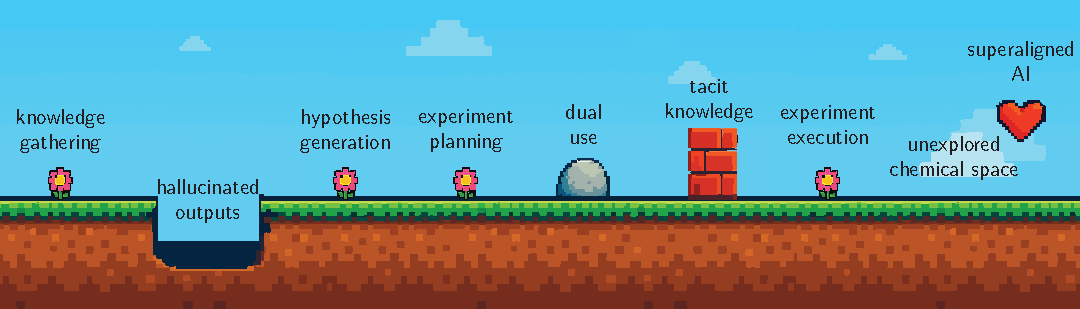
\includegraphics[width=1\linewidth]{figures/safety_chemrev_fig.pdf}
    \caption{\textbf{A conceptual schematic depicting \gls{ai} risk factors in chemical science}. As one traverses through the scientific process, illustrated as a game, there are various obstacles to encountering \gls{ai} exacerbated risks. The path to superaligned chemical \gls{ai}-assistants is obfuscated by unexplored chemical space.}
    \label{fig:safety-overview}
\end{figure}

\noindent \glspl{gpm} in chemistry are double-edged: they accelerate discovery while potentially amplifying chemical safety risks. From democratizing hazardous synthesis knowledge to enabling autonomous dangerous compound production, these systems lower barriers to misuse (\Cref{fig:safety-overview}). Real-world constraints---specialized equipment, regulated reagents, tacit expertise---currently limit risks, but \glspl{gpm} are progressively overcoming these barriers.

\subsubsection{Chemical-Specific Risk Amplification}

\paragraph{Information Access and Synthesis Planning} 
\glspl{gpm} can lower cognitive barriers to accessing dangerous chemical knowledge. \textcite{urbina2022dual} demonstrated that molecular generators like \modelname{MegaSyn} could design toxic agents including VX when reward functions prioritize toxicity. Recent evaluations of \modelname{GPT-4} and \modelname{Claude 4 Opus} for biological threat creation found that while information is already accessible, \glspl{gpm} improve troubleshooting and help acquire tacit knowledge previously limiting non-experts.\autocite{openai2024building, anthropic2025system} \textcite{he2023control} showed \glspl{llm} generate pathways for explosives (\gls{petn}) and nerve agents (sarin). While precursor supply chains remain regulated, \glspl{gpm} that incrementally lower technical barriers act as force multipliers for malicious actors. Chemistry-specific agents like \modelname{ChemCrow}\autocite{bran2024augmenting} and \modelname{Coscientist}\autocite{boiko2023autonomous} demonstrate how \glspl{gpm} can plan and execute complex syntheses---capabilities extending to dangerous compounds.

\paragraph{Hallucinations in Chemical Contexts} 
\glspl{gpm} can hallucinate non-existent reactions, falsify safety protocols, and generate plausible-sounding but incorrect procedures.\autocite{pantha2024challenges, ji2023survey} In chemistry, these errors risk laboratory accidents or synthesis failures that waste resources. Temporal misalignment due to static training data means chemical knowledge becomes outdated as new reactions, hazards, and regulations emerge.

\paragraph{Autonomous Laboratory Risks} 
Autonomous laboratories controlled by \glspl{gpm} face cybersecurity vulnerabilities. Compromised systems could be manipulated to synthesize hazardous compounds. The timeline mismatch between \gls{ai} capabilities and infrastructure security creates risk windows where adversaries exploit inadequately protected systems.\autocite{rouleau2025risks, dean2025security}


\subsubsection{Existing Approaches to Safety} Red-teaming evaluations identify vulnerabilities but are reactive, not preventive. \modelname{ChemCrow}'s safeguards block known controlled substances, yet \textcite{he2023control} demonstrated these protections rely on post-query web searches rather than embedded constraints---easily circumventable. Machine unlearning attempts to remove hazardous knowledge face fundamental challenges in chemistry: defining \enquote{dangerous chemical knowledge} is context-dependent (bleach is benign alone, hazardous when combined), and removal risks degrading model utility for legitimate research. Alignment through \gls{rlhf} reduces harmful outputs but remains vulnerable to jailbreaks\autocite{kuntz2025os-harm, yona2024stealing, lynch2025agentic} and fails to generalize to novel threats (models might refuse known toxins while suggesting precursors).


\subsubsection{Solutions}

Chemical \gls{gpm} oversight should focus on \enquote{advanced chemical models} meeting specific risk thresholds: models trained on sensitive synthesis data, systems demonstrating autonomous synthesis planning capabilities, or agents with laboratory control interfaces. This targeted approach avoids burdening low-risk research while capturing concerning systems---analogous to proposed biological model regulations.\autocite{bloomfield2024ai}

Developing chemistry-aware guardrails requires systems that evaluate chemical plausibility, safety, and regulatory compliance before providing synthesis information. These technical safeguards should integrate real-time hazard assessment checking outputs against controlled substance databases, context-aware refusal mechanisms understanding legitimate versus dangerous use cases, precursor tracking identifying suspicious synthesis pathway queries, and audit logging enabling forensic analysis of concerning interactions. Establishing review processes for \gls{gpm}-assisted chemical research analogous to institutional biosafety committees provides essential institutional oversight. Researchers deploying chemical \glspl{gpm} with autonomous capabilities should undergo safety review, particularly for autonomous synthesis planning and execution, large-scale screening for bioactive compounds, or novel chemical class exploration without expert oversight.

International coordination remains critical for effective chemical \gls{gpm} governance. Unlike self-regulation, which risks conflicts of interest and competitive pressure toward laxity, an international oversight body---analogous to organizations governing nuclear materials or biological weapons---could harmonize safety standards across jurisdictions. Such an \gls{iaio} comprising \gls{ai} researchers, chemists, policymakers, and security experts could establish pre-approval requirements for high-risk chemical \gls{gpm} development, similar to institutional review boards in biomedical research.\autocite{trager2023international} Precedents exist in \gls{cern}'s approach to balancing civilian research with dual-use risk management and nuclear non-proliferation treaties tying market access to compliance.

Transparency requirements should mandate that chemical \gls{gpm} developers publicly report red-teaming results for dangerous synthesis queries, safety evaluation methodologies and thresholds, known vulnerabilities and mitigation strategies, and training data sources documenting chemical knowledge scope. The fundamental tension remains: \glspl{gpm} optimize reactions or design toxins with equal facility, but their black-box nature complicates accountability. Progress requires not just safeguards but deliberate constraints on chemical \gls{gpm} capabilities in high-risk domains.


\subsection{Ethics} \label{sec:ethics}

\gls{gpm} deployment in chemistry raises ethical concerns requiring careful consideration: from bias in chemical knowledge to environmental costs of computation.\autocite{crawford2021atlas}


\subsubsection{Environmental Impact of GPMs}

The computational requirements for training and deploying \glspl{gpm} contribute to environmental degradation through excessive energy consumption and carbon emissions. \autocite{spotte-smith2025considering, nature2023carbon} 
These computational resources are often powered by fossil fuel-based energy sources, which directly contribute to anthropogenic climate change. \autocite{strubell2019energy} 
The emphasis on \gls{ai} research has superseded some commitments made by big technological companies to carbon neutrality. 
For example, Google rescinded its commitment to carbon neutrality amid a surge in \gls{ai} usage (65$\%$ increase in carbon emissions between 2021--24) and funding.\autocite{bhuiyan2025google} 
Additionally, the water consumption for cooling data centers that support these models is another concern, particularly in regions facing water scarcity. \autocite{mytton2021data}

The irony is particularly stark when considering that in the chemical sciences, these models are used to address climate-related challenges, such as the development of sustainable materials or carbon capture technologies. 
As a scientific community, we must grapple with the questions about the sustainability of current \gls{ai} development trajectories and consider more efficient and renewable approaches to model development and deployment. \autocite{kolbert2024obscene}


\subsubsection{Copyright Infringement and Plagiarism Concerns}

\glspl{gpm} are typically trained on a vast corpora of copyrighted scientific literature, patents, and proprietary databases, often without explicit permission, a practice that has sparked legal disputes, such as \textit{Getty Images v.\ Stability \gls{ai}}, where plaintiffs allege unauthorized scraping of protected content. \autocite{kirchhubel2024intellectual} Developers at \modelname{OpenAI} claimed in a statement to the \gls{uk} House of Lords that training \gls{sota} models is \enquote{impossible} without copyrighted material, highlighting a fundamental tension between \gls{ip} law and \gls{ai} advancement. \autocite{openai2023written} 
In the chemical sciences, this challenge persists through the training of models on experimental results from pay-walled journals. 
A potential resolution to this in the scientific sphere lies in the expansion of open-access research frameworks. 
Initiatives like the \gls{cas} Common Chemistry database provide legally clear training data while maintaining attribution.
\glspl{llm} have shown a high propensity to regurgitate elements from their training data. 
When generating text, models may reproduce near-verbatim fragments of training data without citation, effectively obscuring intellectual contributions.\autocite{bender2021dangers} 
While some praise \glspl{gpm} for overcoming \enquote{blank-page syndrome} for early-career scientists \autocite{altmae2023artificial}, others warn that uncritical reliance on their outputs risks eroding scientific rigor.\autocite{donker2023dangers}


\subsubsection{Biases}

\glspl{gpm} inherit and amplify harmful prejudices and stereotypes present in their training data, which pose significant risks when applied translationally to medicinal chemistry and biochemistry. \autocite{spotte-smith2025considering, yang2024demographic, omiye2023large} 
These models can perpetuate inaccurate and harmful assumptions based on race and gender about drug efficacy, toxicity, and disease susceptibility, leading to misdiagnosis and mistreatment. \autocite{chen2023algorithmic} 
Historical medical literature contains biased representations of how different populations respond to treatments, and \glspl{gpm} trained on such data can reinforce these misconceptions. \autocite{mittermaier2023bias}
The problem extends to broader contexts in chemical research. 
Biased models can influence research priorities, funding decisions, and the development of chemical tools in ways that systematically disadvantage the most vulnerable populations \autocite{dotan2019value0laden}. 

\paragraph{Solutions} The problem of bias can be best addressed through top-down reform. 
The data necessary to train unbiased models can only exist if clinical studies of drug efficacy are conducted on diverse populations in the real world.\autocite{criado-perez2019invisible} 
To complement improved data collection, standard evaluations for bias testing must be developed and mandated prior to deployment of \glspl{gpm}.


\subsubsection{Access and Power Concentration} 

Although \glspl{gpm} have the potential to democratize access to advanced chemical research capabilities, they may also concentrate power in the hands of a few large companies that control the frontier models. 
This concentration raises concerns about equitable access to research tools, particularly for researchers in smaller institutions with limited resources.\autocite{satariano2025a1i1}

As a community, we should ensure that the benefits of \glspl{gpm} in chemistry remain broadly accessible via public compute, open-weight models, and portable tooling. We should also insist on fair access terms and transparent benchmarks so that no single provider can gatekeep core research.



